\chapter{Work Completed}
The goal is to find which combination of new techniques provides the greatest overall segmentation results. To that end we have taken a particularly challenging data set, the 2D EM segmentation challenge \cite{emdata}. The training data is a set of 30 sections from a serial section Transmission Electron Microscopy (ssTEM) data set of the Drosophila first instar larva ventral nerve cord (VNC). The microcube measures 2 x 2 x 1.5 microns approx., with a resolution of 4x4x50 nm$/$pixel. The corresponding binary labels are provided in an in-out fashion, i.e. white for the pixels of segmented objects and black for the rest of pixels (which correspond mostly to membranes). This data set has many fine lines to segment, is heavily biased towards the membrane class, and has few training examples. The test set for the model does not have ground truth labels released to the public and instead one must submit their predictions for an accuracy measure. Because of this our result figures can only show our predictions and no ground truth label to compare next to it.

\section{Models}
Here we describe the models we have used for results so far. The overall basic shape of the model is shown in Fig.~\ref{f:model} and the individual components are shown in Fig.~\ref{f:modelpieces}. The overall shape was inspired by the U-Net model from Section~\ref{s:unet}. Instead of using any type of pooling layers we instead use a strided convolution to down sample feature maps. Also we differ from the U-Net model in the short connections. In U-Net the feature maps forwarded by the short connections are concatenated, but in our model they are summed. Along with the residual connections inside each ResBlock, these long residual connections make our model a fully residual model. The full residual model is shown to help information flow within and across levels in the network \cite{quan2016fusionnet}. Also by not concatenating we reduce the number of feature maps in the expanding path of the model. For the multi-scale residual block we hope to increase the models spatial contiguity by giving it multiple fields of view around each local point.

The first half of the network is called the encoding path. Along this path the number of feature maps is doubled after each downsampling. After the center ResBlock begins the decoding path. In the decoding part, the number of feature maps is halved per level to maintain the network symmetry. The downsampling and upsampling are done with convolution layers. These convolutional layers serve as a connector to bridge the input feature maps and the residual block because the number of feature maps from the previous layer may differ from that of the residual block. The proposed network performs an end-to-end segmentation from the input data to the final prediction of the segmentation. We train the network with image set pairs corresponding to the image and its segmentation label, compare the output with manual segmentation, and use a loss function to back-propagate to adjust the weights of the network.

\begin{figure}[h!]
	\centering
		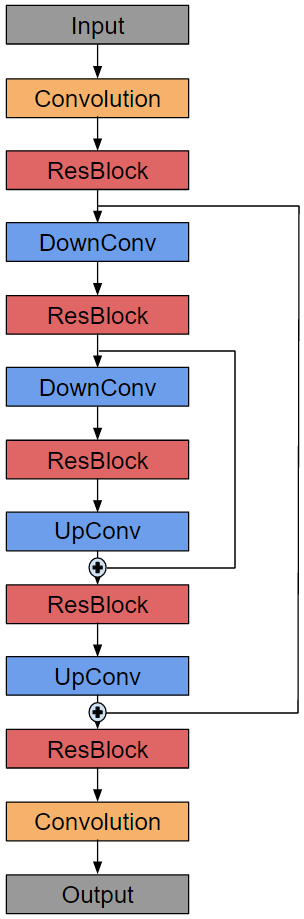
\includegraphics[width=0.4\textwidth]{figures/mymodel.png}
	\caption{The model architecture. Feature maps from the down path get summed with feature maps of the corresponding size in the up path. The ResBlock types are shown in Figs.~\ref{f:basic}~\&~\ref{f:multi} and the DConvolution and UConvolution are shown in Fig.~\ref{f:dconv} and Fig.~\ref{f:uconv} respectively.}
	\label{f:model}
\end{figure}
\begin{figure}
    \centering
    \begin{subfigure}[b]{0.39\textwidth}
        \centering
        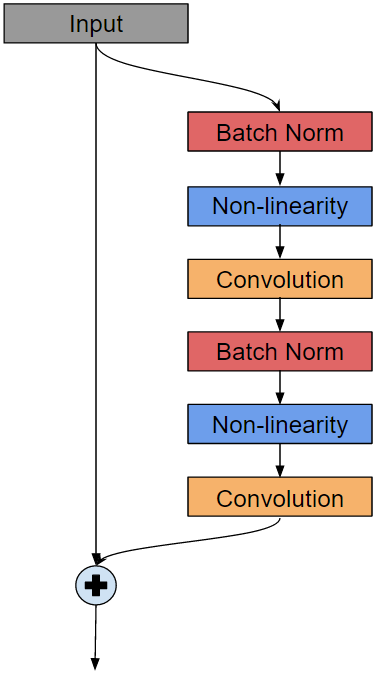
\includegraphics[width=\textwidth]{figures/basic.png}
        \caption{A basic residual block.}
				\label{f:basic}
    \end{subfigure}
    \hfill
		\begin{subfigure}[b]{0.59\textwidth}
        \centering
        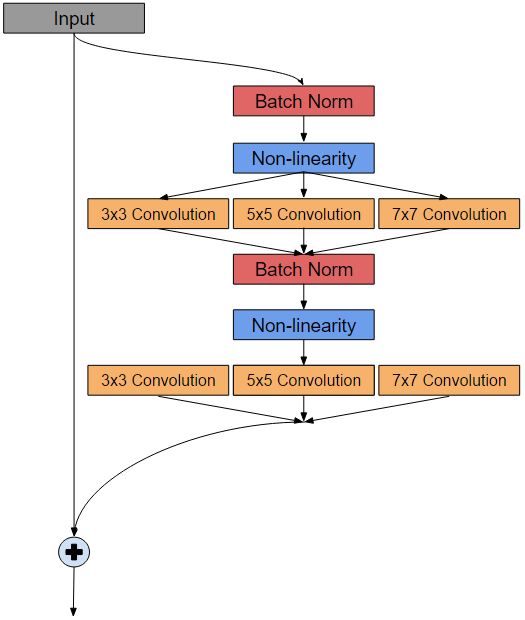
\includegraphics[width=\textwidth]{figures/multiscale.png}
				\caption{A multi-scale residual block.}
        \label{f:multi}
    \end{subfigure}
    \\
    \begin{subfigure}[b]{0.25\textwidth}
        \centering
        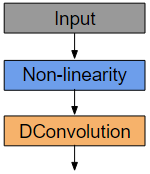
\includegraphics[width=\textwidth]{figures/dconv.png}
				\caption{A down sampling block.}
        \label{f:dconv}
    \end{subfigure}
    \hfill
    \begin{subfigure}[b]{0.25\textwidth}
        \centering
        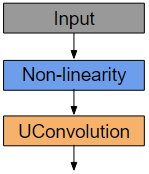
\includegraphics[width=\textwidth]{figures/uconv.png}
				\caption{An upsampling block.}
        \label{f:uconv}
    \end{subfigure}
    \caption{Model components.}
    \label{f:modelpieces}
\end{figure}

\section{Training}
For training we select an image size $s$ and a batch size $B$. We then randomly sample a $s\times s$ image from a randomly selected training image. That sub-image is then modified by first adding a very small amount of Gaussian noise, randomly flipped left to right or top to bottom, and randomly rotated a small angle between -20 and 20 degrees. Sub-images are grabbed in this manner until there are $B$ of them. The batch is then run through the model and the weights are updated. We have a set number of batches that we called an epoch, but each epoch is a different set of batches since all augmentation happens online. After each epoch we observe the model's loss on the validation set and keep a record of it along with the corresponding weights. After the total number of epochs is done running we restore the weights to the point of lowest validation loss.

\section{Experimental Setup}
The proposed deep network is implemented using Keras open-source deep learning library \cite{chollet2015}. This library provides an easy-to-use high-level programming API written in Python, and Theano or TensorFlow can be chosen for a backend deep learning engine. Since the work was done on a Windows PC the Theano backend was chosen as TensorFlow did not support GPU processing on Windows. Training and deployment of the network is conducted on a PC equipped with an Intel i7 CPU with a 64 GB main memory and an NVIDIA GTX Geforce 980 Ti GPU.

\section{Results}
This section will show comparison results from many different models so we will break this section into subsections and begin each subsection with a description of the models being compared. 

\subsection{Basic Comparison}
In this section we are establishing a baseline for each of the three main models. We are comparing: the U-Net \cite{ronneberger2015u}, our model shown in Fig.~\ref{f:model} with the basic residual block shown in Fig.~\ref{f:basic}, and our model shown in Fig.~\ref{f:model} with the multi-scale residual block shown in Fig.~\ref{f:multi}. This baseline is using the most common non-saturating activation function, the ReLU shown in Eq.~\ref{e:relu}. Also we did not apply Batch Normalization in any of these baseline models. The loss function used was a binary cross-entropy on each pixel of the output. The loss plots are shown in Fig.~\ref{f:baseline-loss} and a sample segmentation is shown in Fig.~\ref{f:baseline}.

\begin{figure}[h!]
	\centering
		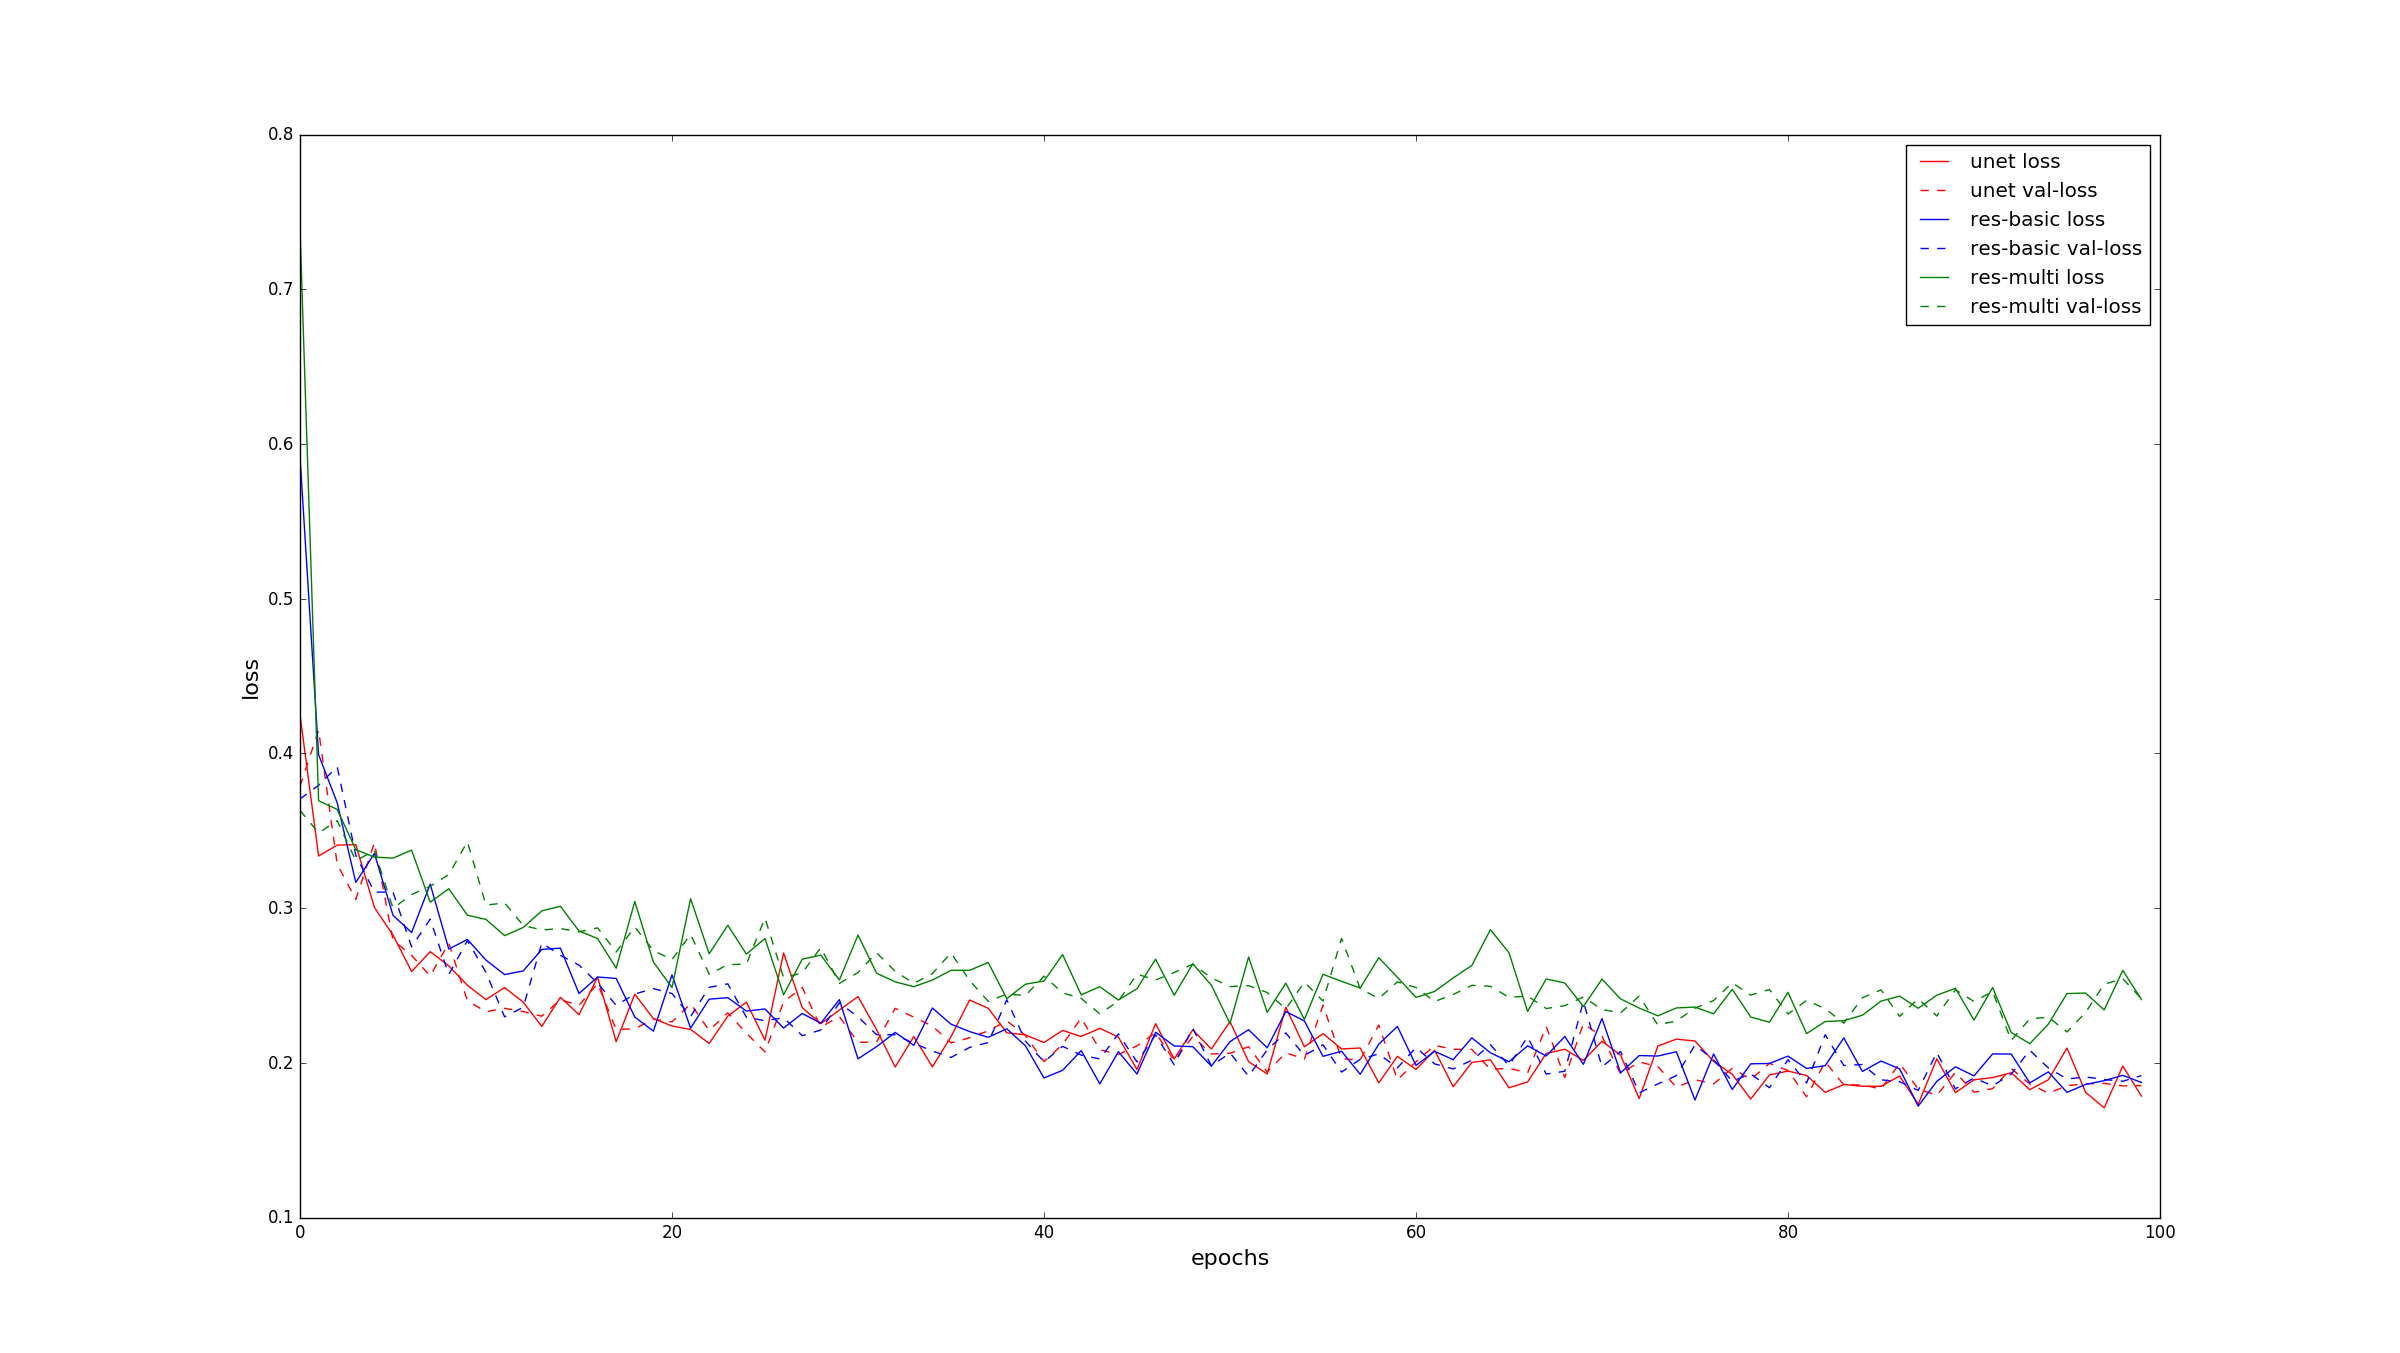
\includegraphics[width=1.0\textwidth]{figures/baseline_loss.png}
	\caption{The loss and validation loss during training for the baseline models.}
	\label{f:baseline-loss}
\end{figure}
\begin{figure}[h!]
	\centering
		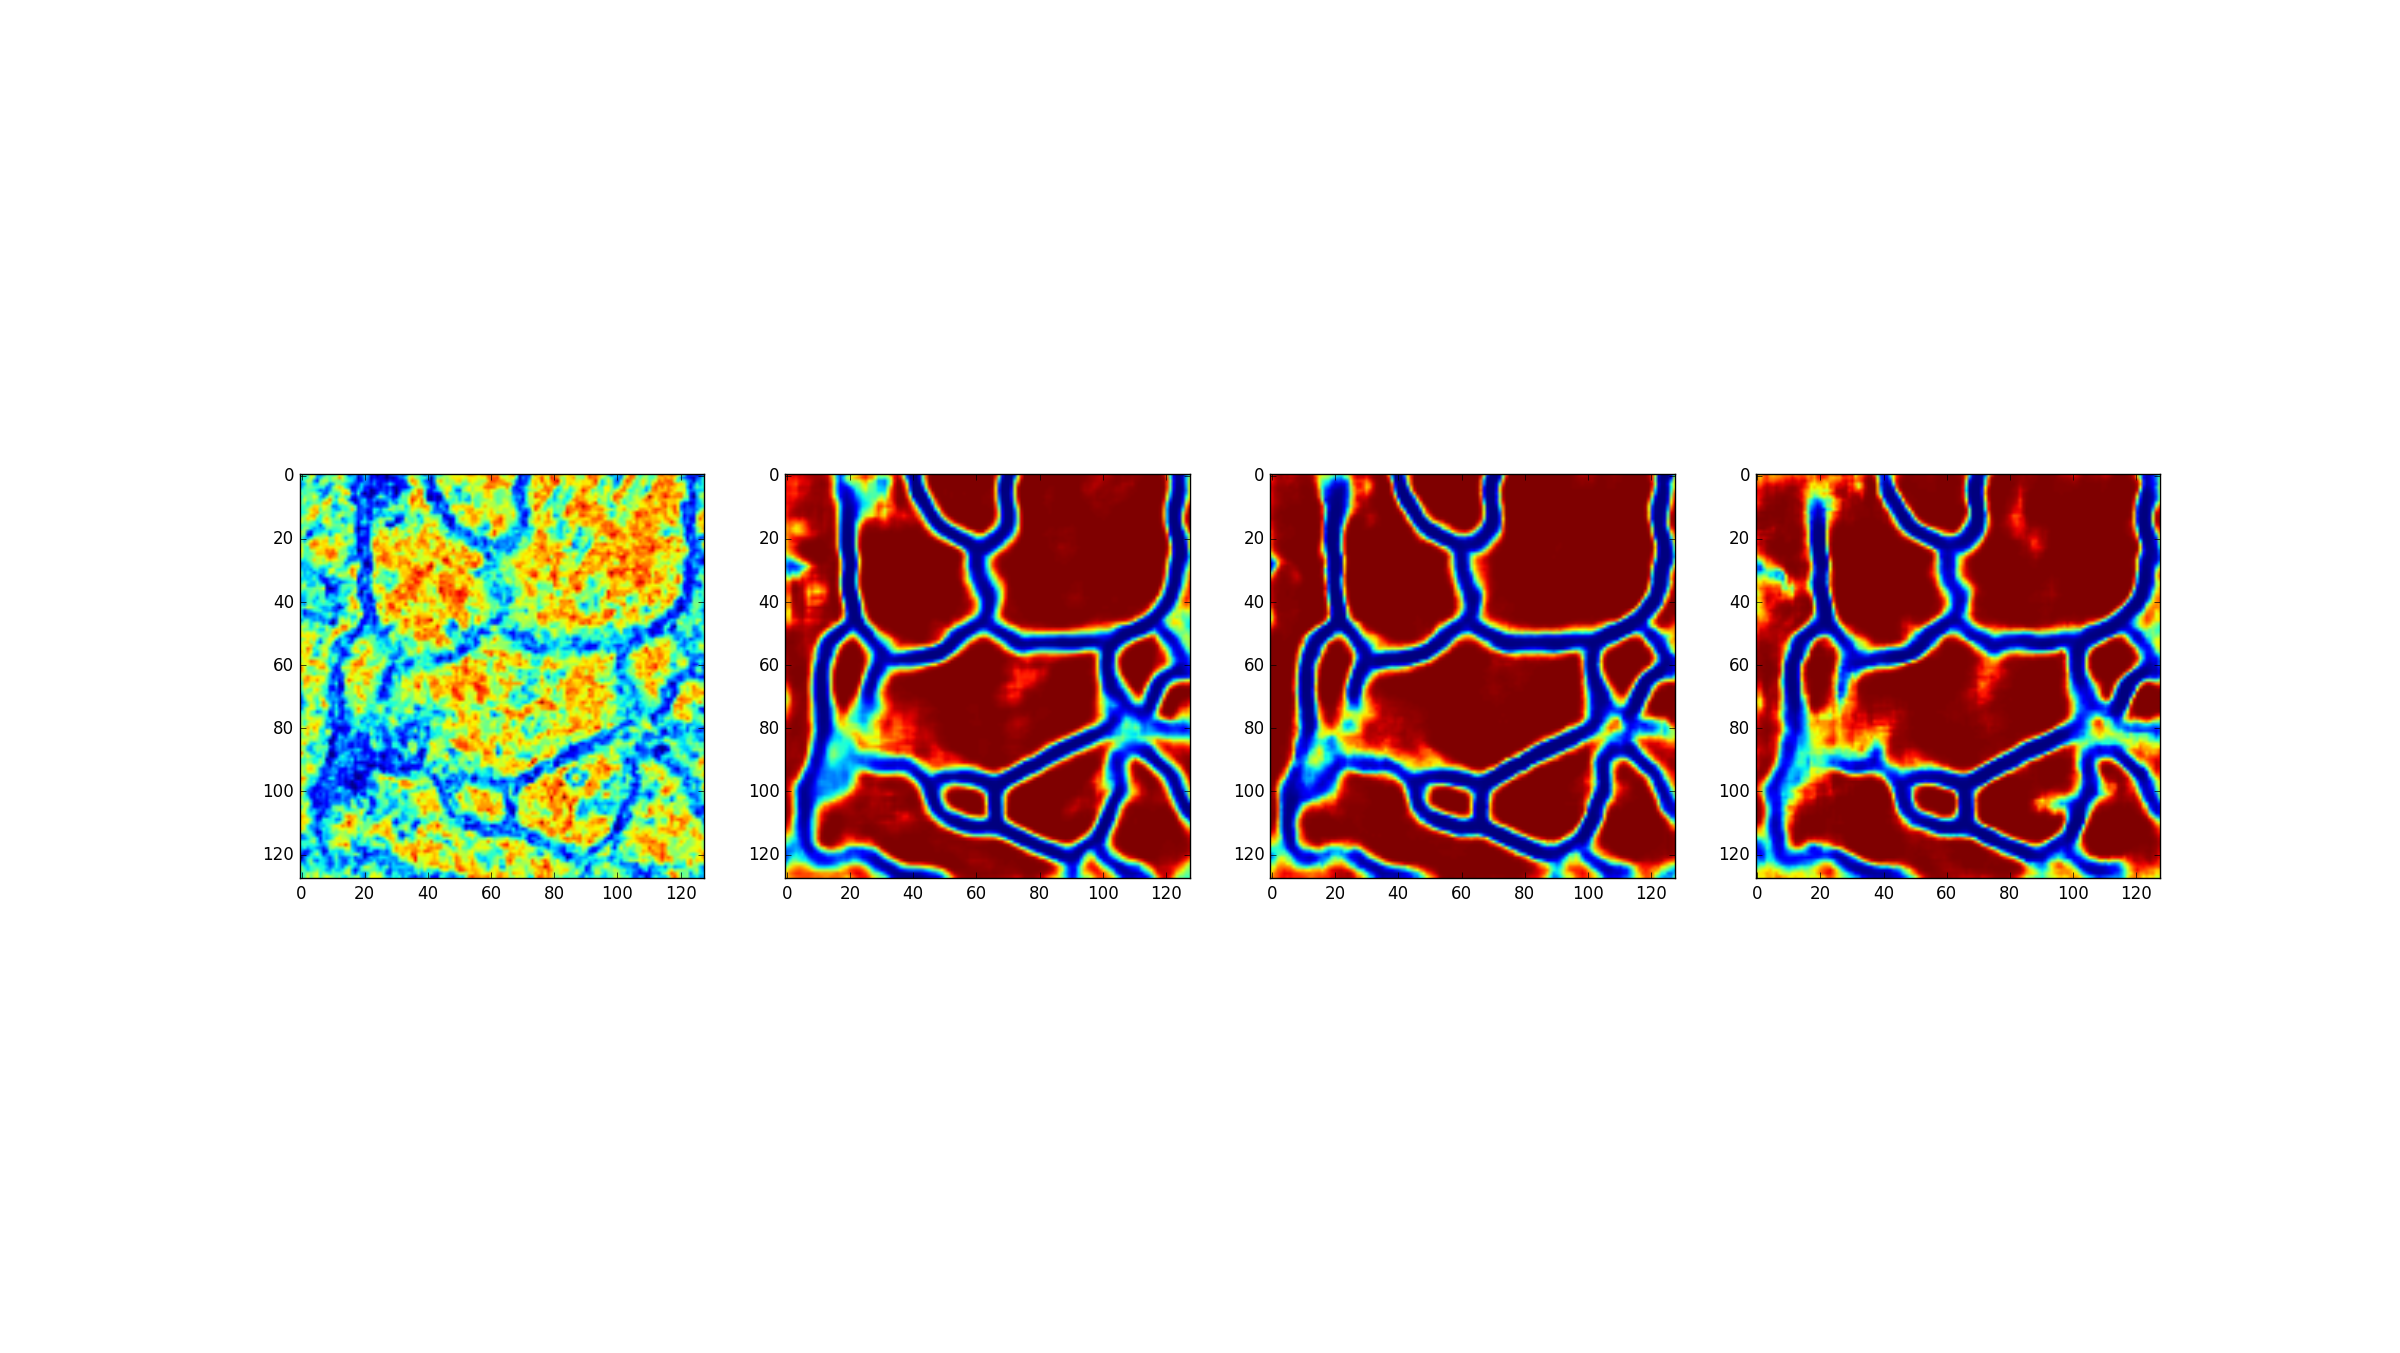
\includegraphics[width=1.0\textwidth]{figures/baseline.png}
	\caption{Sample segmentation on a test image for the baseline models. The test image is shown in its normalize stated, which is scaling the values between minus one and one. From left to right: test image, U-Net segmentation, our model, and our model with multi-scale convolution. The segmentations are shown in a red to blue color map where red is 0 and blue is 1.}
	\label{f:baseline}
\end{figure}

\subsection{Applying Batch Normalization}
Most state of the art models use Batch Normalization. We apply it directly before every non-linearity in the model. This is to keep the values, which can become large from the addition operations of the residual connections, stay mean centered. The loss plots are shown in Fig.~\ref{f:batchnorm-loss} and a sample segmentation is shown in Fig.~\ref{f:batchnorm}. Compare how smooth the losses are compared to the baseline model's loss in Fig.~\ref{f:baseline-loss}. The resulting segmentations also come out much more crisp, especially around the edges of the membranes compared to the basic model's segmentation in Fig.~\ref{f:baseline}. Another interesting observation is that the multi-scale segmentation completely segmented the large membrane structure in the bottom right, while the other two models left the center open. This shows that the wider field of view helped the multi-scale model in this instance.

\begin{figure}[h!]
	\centering
		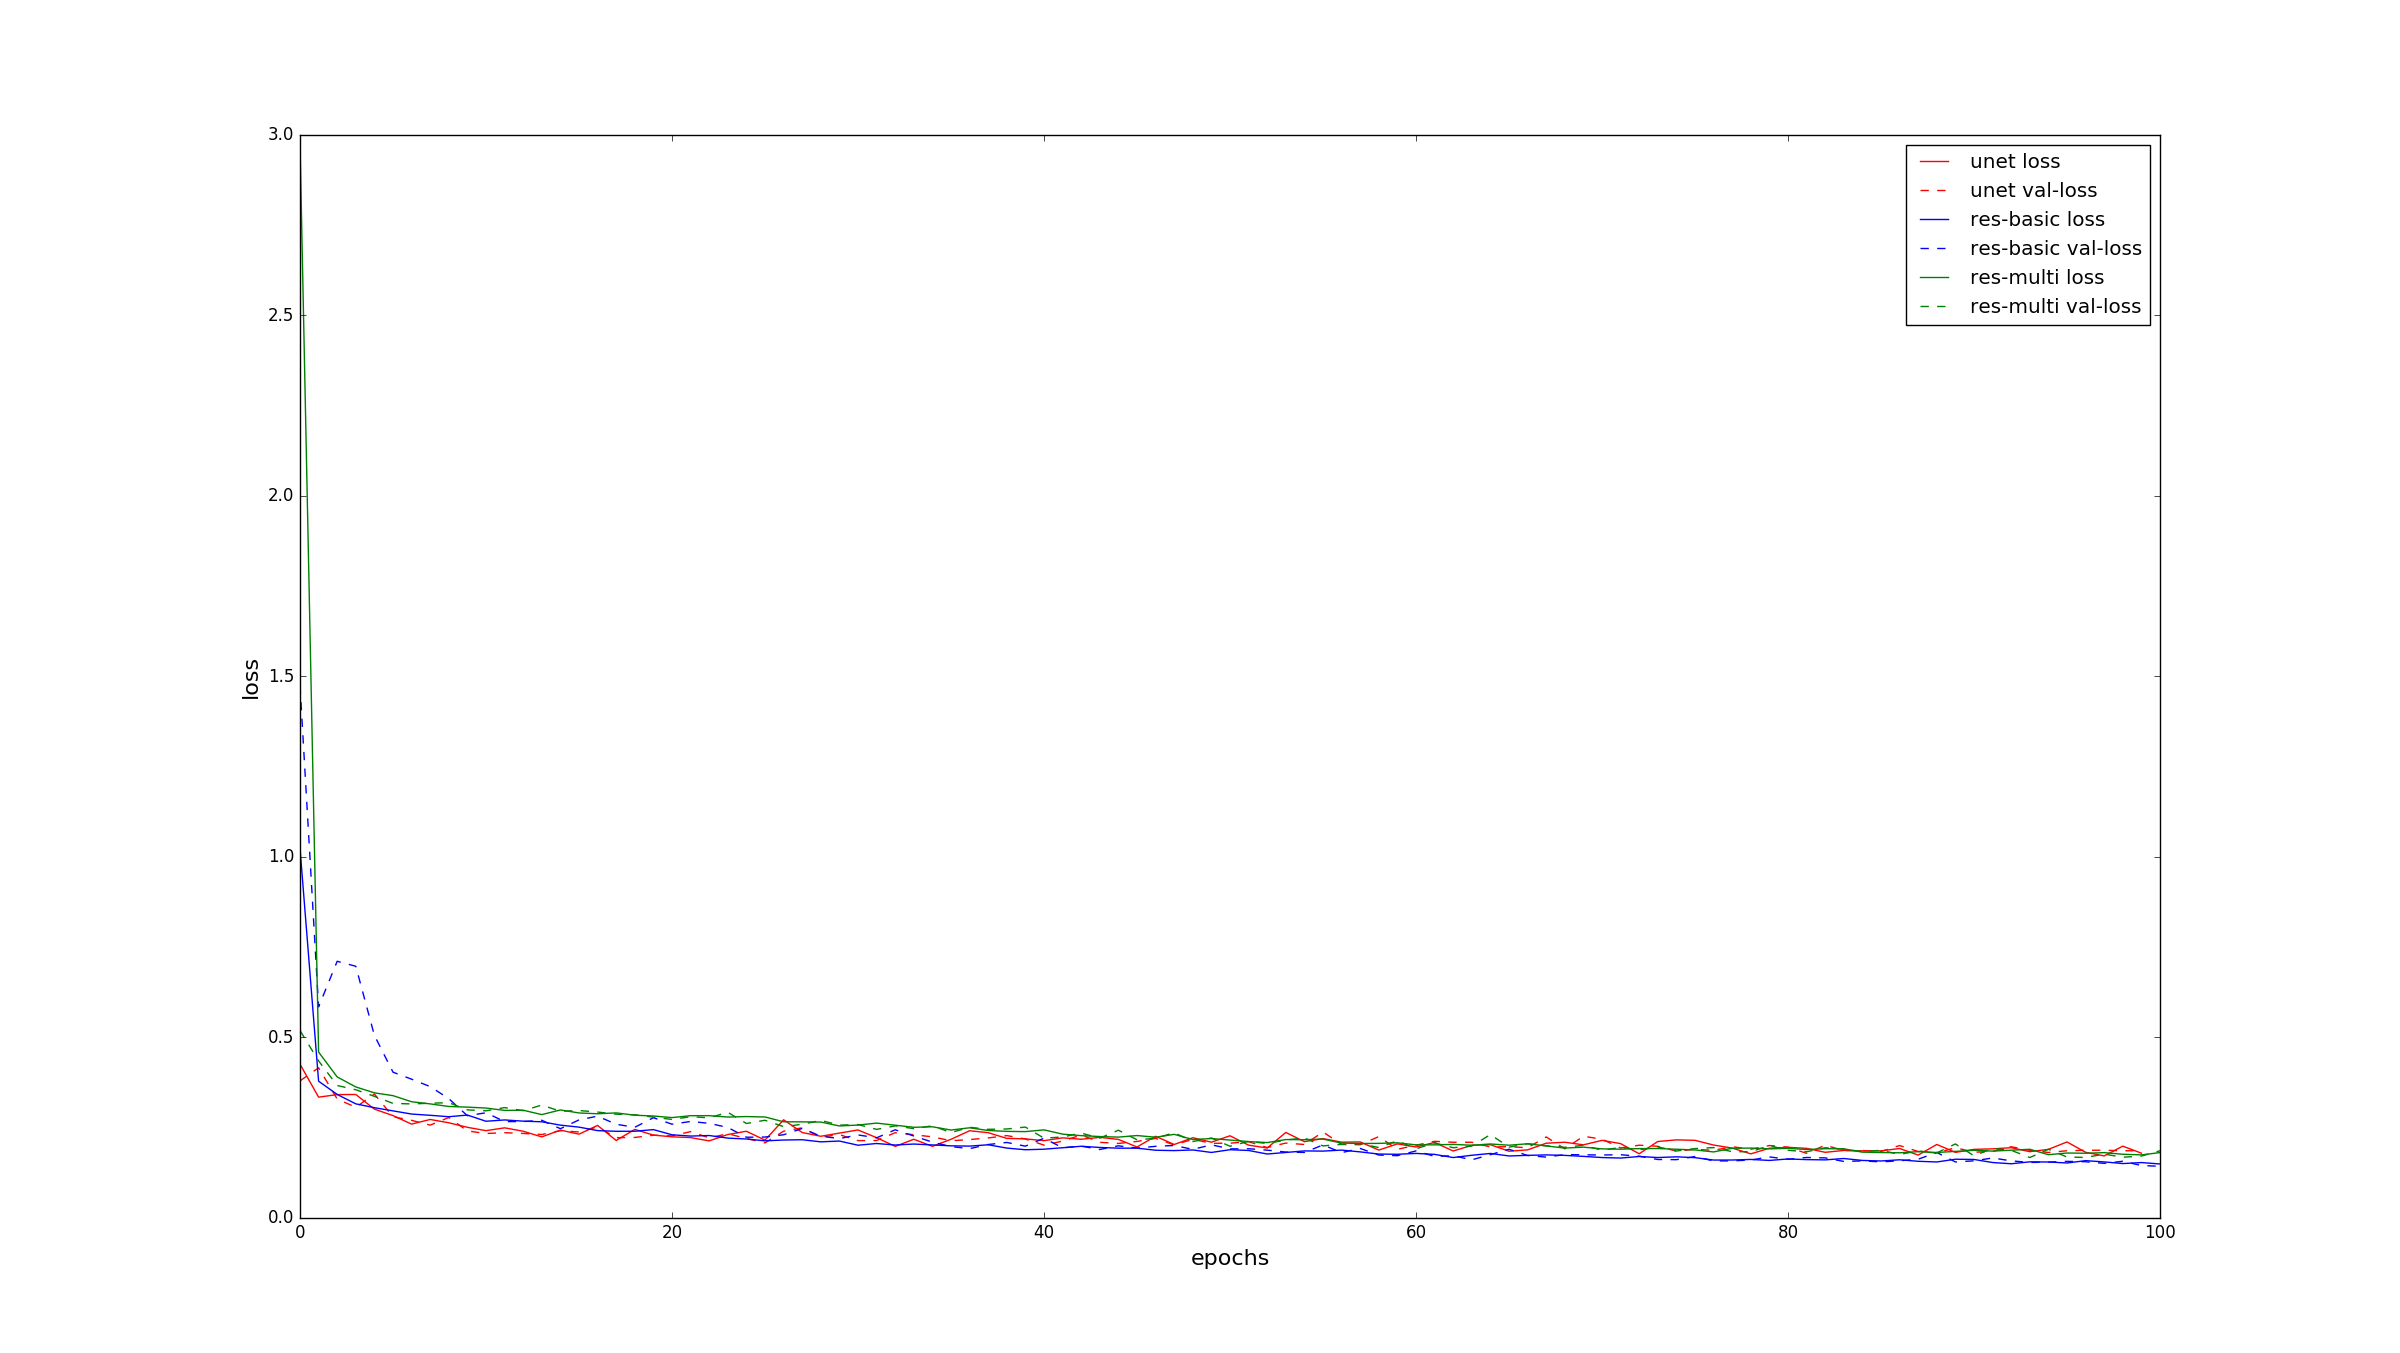
\includegraphics[width=1.0\textwidth]{figures/batchnorm_loss.png}
	\caption{The loss and validation loss during training for the batchnorm models.}
	\label{f:batchnorm-loss}
\end{figure}
\begin{figure}[h!]
	\centering
		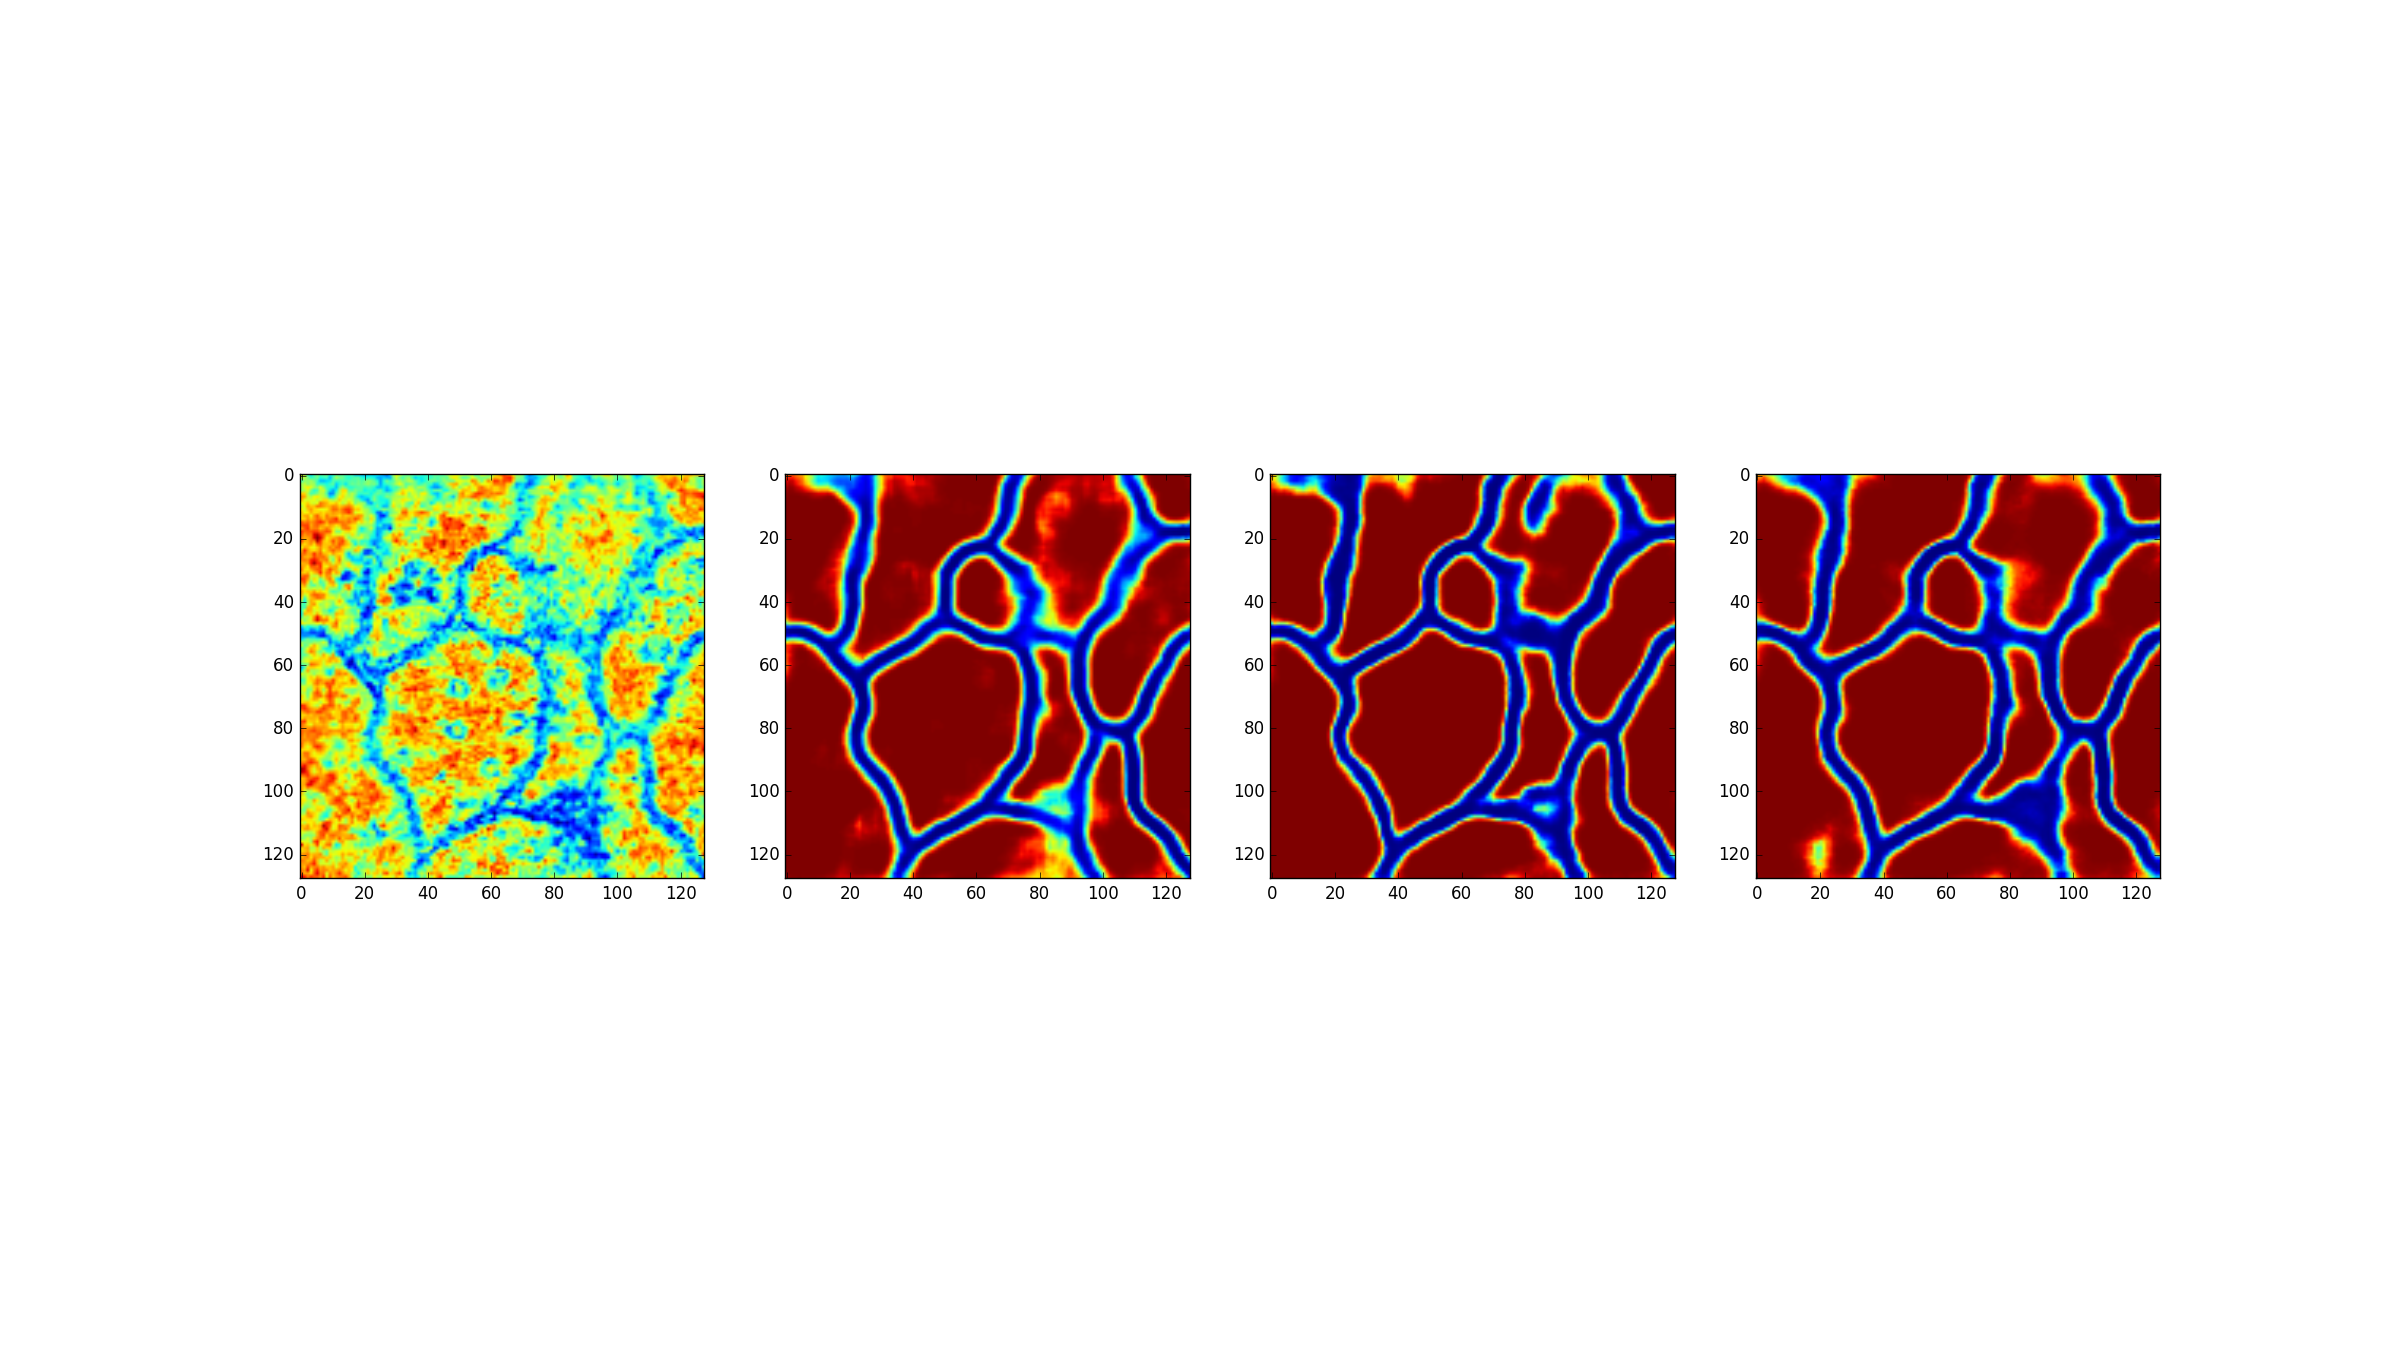
\includegraphics[width=1.0\textwidth]{figures/batchnorm.png}
	\caption{Sample segmentation on a test image for the batchnorm models. From left to right: test image, U-Net segmentation, our model, and our model with multi-scale convolution.}
	\label{f:batchnorm}
\end{figure}

\chapter{Additional Research}
In the above we have explored the effects of combining several new breakthroughs in deep neural networks for the task of semantic segmentation. Going forward we would like to explore using GAN models using the newly proposed Wasserstein and the least square loss functions to combat the training instabilities often seen in GANs. This would be the first to our knowledge implementation of GANs for segmentation with those loss functions. We would use the models we have already explored as the generators for these GANs and could publish a stand alone paper on these results.

We also want to look at the results of running a RNN refinement type model on the outputs of all previous models we have explored as well as the GANs outputs. While this may improve our GANs results, we do not believe it would be enough for its own paper.

We also intend to run all of models on more data sets. For the second data set we chose the Larval Zebrafish EM data, which is another neuronal segmentation challenge. However, this set has released the ground truth labels for the test data. And lastly we want to run on a more natural image challenge so we chose the COCO 2016 Detection Challenge segmentation challenge. The COCO data set has more than 200,000 images and 80 object categories.


\chapter{Timeline}
The additional research to be carried out could be finished over the summer months. The code base is written in a very modular way allowing changes to any part of the models with a single variable change. 

\section{Refinement RNN}
The code for the refinement RNN is already written, but no results have been generated yet. The biggest challenge with this model is that it requires a large amount of GPU memory and it takes a long time to train compared to the other models in this paper. To combat this we intend to deploy this model on AWS instances so it does not tie up my main machine from other work. I am very familiar with using AWS so the setup time will be very minimal.

\section{GAN Model}
The majority of the time will come from the implementation of the GAN model. For only this model we will need to add some new code that handles training the discriminator and generator in simultaneous fashion. We also must implement the proposed loss functions since they are not build into any existing deep learning framework. We plan to attack this problem in steps. First we will implement a simple GAN to generate MNIST examples in a too be determined deep learning framework. Once this is working we will create the new loss functions and test them on the MNIST GAN. After we are confident in our ability to run the simultaneous training steps and that our custom loss functions are working we will implement the segmentation GAN.